Sistemas de 1ª ordem, normalizados, são do tipo:

$$G(s) = \frac{a}{s+a}$$

\section{Resposta ao Degrau}

Sabendo o polo $a$ do sistema é possível traçar sua resposta em degrau utilizando a resposta padrão:

$$y(t) = (1 - e^{-at})u(t)$$

Outras informações que podemos obter são a \textit{constante de tempo $\tau$} e o \textit{tempo de estabilização $T_{s}$}.

A constante de tempo é definida por:

$$\tau = \frac{1}{a}$$

O tempo de estabilização(para um erro de $2\%$) é dado por:

$$T_{s} = \frac{4}{a}$$

\begin{example}
Encontre as características e a resposta ao degrau de um sistema cujo a função de transferência é dada por:
$$G(s) = \frac{2}{s+2}$$
\end{example}
\vspace{20mm}
\textbf{O código da resolução está na próxima página}
\newpage

\begin{lstlisting}
s=%s;
G = 2/(s+2);

//Com a funcao roots eu encontro a raiz(polo) do polinomio s+2
polo = roots(s+2);

//Para encontrar a constante de tempo basta dividir 1/a
cte_tempo = 1/polo;

//Para encontrar o tempo de estabilizacao basta dividir 4/a
t_estabilizacao = 4/polo;

t = 0:0.01:15;

//Para plotar o grafico da resposta ao degrau utilizamos a funcao
y = (1-%e^(polo*t));

plot(t,y)

\end{lstlisting}

Obtêm-se o seguinte gráfico:

\begin{figure}[!htb]
\centering
    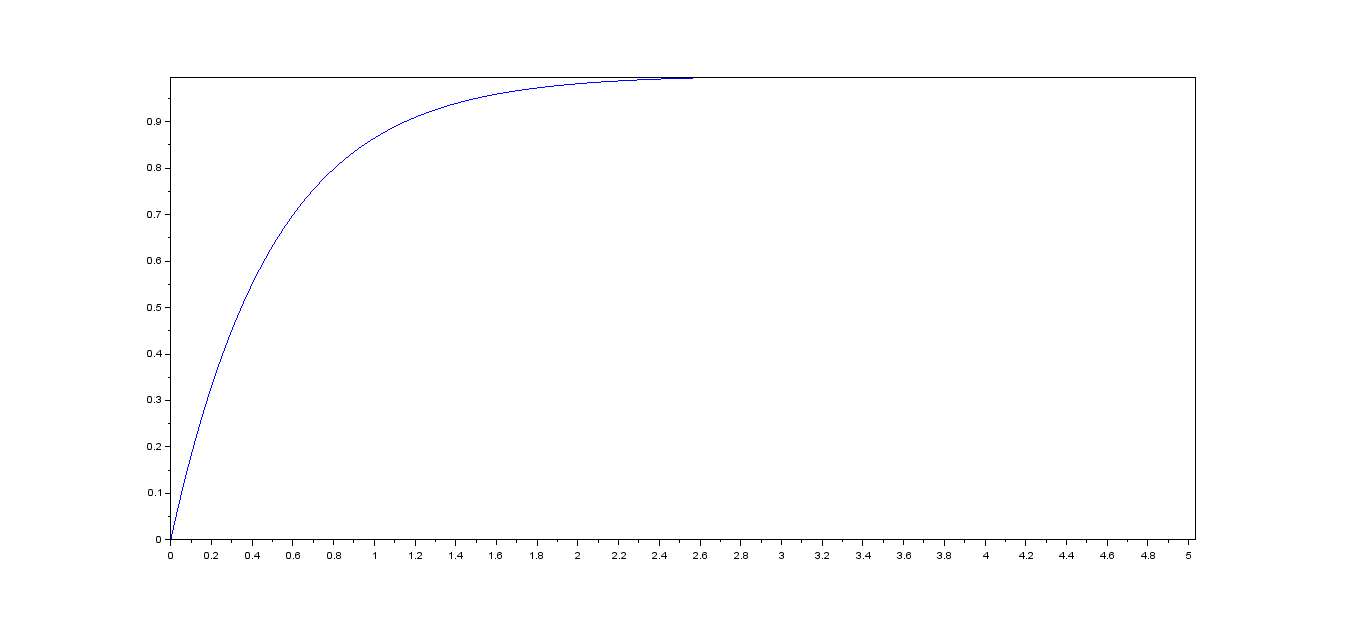
\includegraphics[scale=0.4]{CapitulosPrincipais/RespTransSistContinuos/Imagens/exemplo1.png}
\end{figure}